\documentclass{article}

\usepackage{pandekten}

\usepackage{dashrule}

\makeatletter
\newcommand*{\shifttext}[1]{%
  \settowidth{\@tempdima}{#1}%
  \hspace{-\@tempdima}#1%
}
\newcommand{\plabel}[1]{%
\shifttext{\textbf{#1}\quad}%
}
\newcommand{\prule}{%
\begin{center}%
\hdashrule[0.5ex]{.99\linewidth}{1pt}{1pt 2.5pt}%
\end{center}%
}

\makeatother

\setlength{\parindent}{0pt}

\title{Assignment 2}
\author{Ze Chen}

\begin{document}

\maketitle

\plabel{1}%
The matrix element is given by
\[ \bra{n10} (-ez) \ket{n00} = \frac{\sqrt{3}}{2}\sqrt{n^2(n^2-1)} \approx \frac{\sqrt{3}}{2}n^2. \]
\begin{center}
    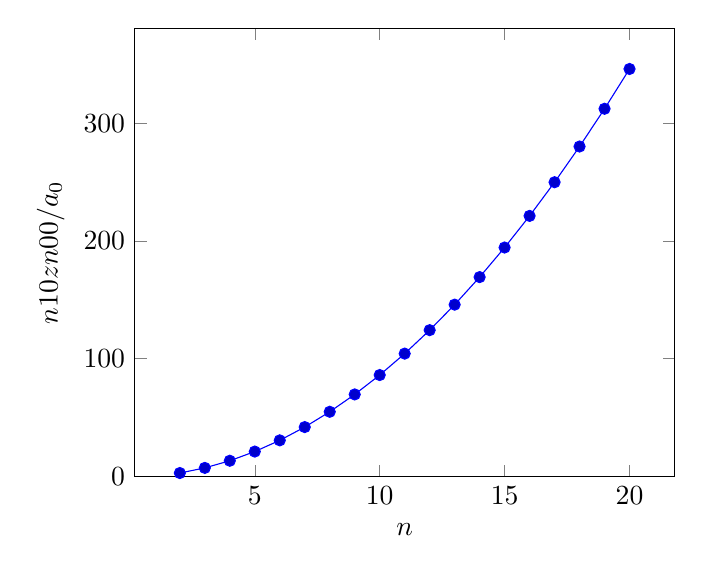
\begin{tikzpicture}
        \begin{axis}[ 
          xlabel={$n$},
          ylabel={$\bra{n10}{z}\ket{n00}/a_0$},
          %xmin=2, xmax=20,
          ymin=0, %ymax=55,
          %xtick={1,...,20},
          domain={2:20},
          samples=19
        ]
          \addplot {sqrt(3)/2*sqrt(x^2 * (x^2 - 1))}; 
        \end{axis}
    \end{tikzpicture}
\end{center}

\prule

\plabel{2 (a)}%
Energy levels are
\[ \ket{0} = \ket{5\mathrm{S}_{1/2},F=1,m_F=0}, \]
and
\[ \ket{1} = \ket{5\mathrm{S}_{1/2},F=2,m_F=0}. \]
\par
Initialization in $\ket{0}$ through Raman-assisted optical pumping.
\par
Read out by pushing atoms in $\ket{1}$ out of the traps with a resonant laser pulse, followed by a site-resolved fluorescence image of the remaining atoms.

\plabel{(b)}%
$X(\theta)$ is implemented with a global drive field generated by a \SI{795}{\nano\meter} laser tuned near the $5\mathrm{S}_{1/2}$ to $5\mathrm{P}_{1/2}$ transition.
\par
$Z(\theta)$ is implemented with stark effect by a local addressing laser.

\plabel{(c)}%
The evolution is given by
\begin{equation}
    \label{eq:initial11}
    i\begin{pmatrix}
        \dot{\alpha}_{11}(t) \\ \dot{\beta}_{11}(t)
    \end{pmatrix} = \Omega \begin{pmatrix}
        0 & \sqrt{2}/2 \\ \sqrt{2}/2 & -\Delta/\Omega
    \end{pmatrix} \begin{pmatrix}
        \alpha_{11}(t) \\ \beta_{11}(t)
    \end{pmatrix}
\end{equation}
with initial condition $\begin{pmatrix}
    \alpha_{11}(0) & \beta_{11}(0)
\end{pmatrix} = \begin{pmatrix}
    1 & 0
\end{pmatrix}$ starting with $\ket{11}$, and
\[ i\begin{pmatrix}
    \dot{\alpha}_{01}(t) \\ \dot{\beta}_{01}(t)
\end{pmatrix} = \Omega \begin{pmatrix}
    0 & 1/2 \exp(i\xi\Theta(t - \tau)) \\ 1/2\exp(-i\xi\Theta(t - \tau)) & -\Delta/\Omega
\end{pmatrix} \begin{pmatrix}
    \alpha_{01}(t) \\ \beta_{01}(t)
\end{pmatrix} \]
with initial condition $\begin{pmatrix}
    \alpha_{01}(0) & \beta_{01}(0)
\end{pmatrix} = \begin{pmatrix}
    1 & 0
\end{pmatrix}$ starting with $\ket{01}$,
where
\begin{align*}
    \Omega &= 2\pi\times \SI{3.5}{\mega\hertz}, \\
    \Delta/\Omega &= \num{0.377}, \\
    \xi &= \num{3.9024},
\end{align*}
and $\tau = \SI{0.195083}{\micro\second}$ is the period from \eqref{eq:initial11}.
The numerical solution is given by Mathematica.
\par
The phase factor is obtained from the numerical solution.
\begin{align*}
    \phi_{01} = \arg \alpha_{01}(2\tau) &= \SI{2.37906}{rad}, \\
    \phi_{11} = \arg \alpha_{11}(2\tau) &= \SI{1.61845}{rad}. \\
\end{align*}
We find that
\[ 2\phi_{01} - \phi_{11} = \SI{3.14}{rad} = \pi. \]

\begin{center}
    \begin{tikzpicture}
        \begin{axis}[xlabel=${\SI[number-math-rm=\mathnormal,parse-numbers=false]{t}{\per\micro\second}}$, ylabel=$\abs{\bra{\beta}\ket{\varphi}}^2$]
        \addplot table {plotB01.txt};
        \addlegendentry{$\ket{01}$};
        \addplot table {plotB11.txt};
        \addlegendentry{$\ket{11}$};
        \end{axis}
    \end{tikzpicture}
\end{center}

\plabel{(d)}%
State preparation and measurement error, finite atomic temperature, and laser scattering during Rydberg dynamics.

\plabel{(e)}%
The truth table measurement is in a rotated basis so that it is more experimentally accessible than full process tomography.

\prule

\plabel{3 (a)}%
In Madjarov et al., the atom is the alkaline-earth atom \ce{^{88}Sr}, while in Levine et al., the atom is the alkali atom \ce{^{87}Rb}.
\par
In Madjarov et al., the effective ground state is the metastable state $\ket{g} = \mathrm{5s5p({^3P_0})}$ and the Rydberg state is $\ket{r} = \mathrm{5s61s({^3S_1})}$. In Levine et al., $\ket{0}$ and $\ket{1}$ are the $^5S_{1/2}$ states and the Rydberg state is $\ket{r} = 70S_{1/2}$.
\par
In Madjarov et al., exitation to the Rydberg state from the effective ground state is a single photon process, while in  Levine et al. it is an two-photon process.

\plabel{(b)}%
They characterize the Bell state fidelity associated with a two-atom blockaded $\pi$-pulse.
\par
Parity oscillations require site-resolved laser addressing while in their experiment all beams are along the axis of the atom array and address all atoms simultaneously.
\par
They did it by measuring the population at $\pi$ and $2\pi$ time to provide a lower bound on the purity of of the two-atom state.

\plabel{(c)}%
The tweezers are switched off during Rydberg excitation.
However, blinking traps on and off will eventually lead to heating and loss and therefore a lower fidelity.

% \bibliographystyle{plain}
% \bibliography{main}

\end{document}
